% Part: sets-functions-relations
% Chapter: relations
% Section: trees

\documentclass[../../../include/open-logic-section]{subfiles}

\begin{document}

\olfileid[fr]{sfr}{rel}{tre}
\olsection{Arbres}

Un \emph{arbre} est un type particulier d’ordre partiel qui joue un rôle
important dans toutes les branches de la logique. Les arbres finis
apparaissent dès la logique élémentaire : les !!{formula}s peuvent ainsi
être analysées au moyen de leur décomposition en arbres syntaxiques,
et les !!{derivation}s, dans de nombreux systèmes de !!{derivation},
prennent elles aussi la forme d’arbres finis.
%
Les arbres infinis interviennent dès la démonstration des théorèmes
de complétude de la logique propositionnelle et de la logique du premier
ordre ; on les retrouve dans toute la logique mathématique.

La notion ensembliste d’arbre est étroitement liée à celle de la théorie
des graphes. Voici la représentation d’un arbre fini :

\begin{center}
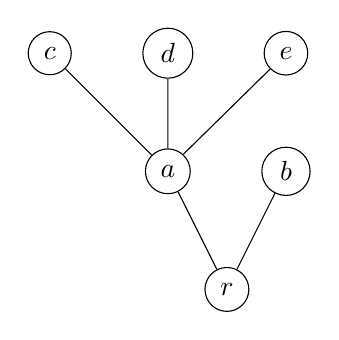
\begin{tikzpicture}[nodes={draw, circle}, -]
\node{$r$} [grow'=up]
    child { node {$a$}
        child { node {$c$} }
        child { node {$d$} }
        child { node {$e$} }
    }
    child { node {$b$} };
\end{tikzpicture}
\end{center}

Le nœud~$r$, situé tout en bas, est la racine. Tout nœud autre que $r$
possède exactement un nœud parent immédiatement au-dessous de lui.
On peut interpréter la relation entre un nœud~$x$ et un nœud~$y$ que
l’on atteint depuis~$x$ en suivant les arêtes vers le haut en disant
que $x$ est un \emph{ancêtre} de~$y$.

La relation d’ascendance dans un arbre est un ordre partiel strict.
Cela motive la définition ensembliste. Pour l’énoncer, nous avons besoin
de deux notions. Un \emph{plus petit élément} d’un ensemble~$A$
partiellement ordonné par~$\le$ est !!a{element} $x \in A$ tel que,
pour tout $y \in A$, on ait~$x \le y$. Un ensemble est \emph{bien ordonné}
par~$\le$ si chacune de ses parties non vides possède un plus petit élément.

\begin{defn}[Arbre]
Un \emph{arbre} est un couple $T = \tuple{A, \le}$ où $A$ est un ensemble
et $\le$ un ordre partiel sur~$A$ possédant un unique plus petit élément
$r \in A$, appelé la \emph{racine}, et tel que, pour tout $x \in A$,
l’ensemble $\Setabs{y}{y \le x}$ soit bien ordonné par~$\le$.
\end{defn}

\begin{defn}[Successeurs]
Soit $T = \tuple{A, \le}$ un arbre. Si $x,y \in A$, $x < y$ et
qu’il n’existe aucun $z \in A$ tel que $x < z < y$, on dit que $y$
est un \emph{successeur} de~$x$.
\end{defn}

Les successeurs de $x \in A$ sont aussi appelés ses \emph{enfants}.
Si $y$ est un successeur de~$x$, on dit que $x$ est le \emph{prédécesseur}
ou le \emph{parent} de~$y$.

\begin{prop}
Si $\tuple{A,\le}$ est un arbre, tout $x \in A$ autre que la racine
possède au plus un prédécesseur.
\end{prop}

\begin{proof}
Supposons $y_1 < x$, $y_2 < x$ et $y_1 \neq y_2$.
Alors $\{y_1, y_2\} \subseteq \Setabs{z}{z<x}$.
Puisque $\Setabs{z}{z<x}$ est bien ordonné par~$\le$, sa partie
$\{y_1, y_2\}$ possède un plus petit élément, qui est nécessairement
$y_1$ ou~$y_2$. Ainsi, $y_1 \le y_2$ ou $y_2 \le y_1$.
Or $y_1 \neq y_2$ par hypothèse ; on a donc $y_1 < y_2$ ou $y_2 < y_1$.
Comme $y_1 < x$ et $y_2 < x$, on en déduit que $y_1 < y_2 < x$
ou $y_2 < y_1 < x$. Les deux objets $y_1$ et $y_2$ ne peuvent donc
pas être tous deux des prédécesseurs de~$x$.
\end{proof}

\begin{defn}
Un arbre $T = \tuple{A, \le}$ est dit \emph{infini} si $A$ est infini,
et \emph{fini} sinon. Si chaque $x \in A$ possède un nombre fini
de successeurs, on dit que $T$ est \emph{à branchement fini}.
\end{defn}

\begin{defn}[Branches]
Soit $T = \tuple{A, \le}$ un arbre. Une \emph{branche} de~$T$ est une
chaîne maximale dans~$T$, c’est-à-dire un ensemble $B \subseteq A$
tel que, pour tous $x, y \in B$, on ait $x \le y$ ou $y \le x$,
et que, pour tout $z \in A \setminus B$, il existe $u \in B$ tel que
l’on n’ait ni $z \le u$ ni $u \le z$.\footnote{Correction éditoriale :
le domaine est bien celui de l’arbre. L’original écrivait ici la lettre
$X$, qui n’avait pas été définie, à la place de $A$.}
%
On note $[T]$ l’ensemble de toutes les branches de $T$.
\end{defn}

\begin{ex}
Un exemple classique d’arbre à branchement fini est l’\emph{arbre binaire
infini} des suites finies de $0$ et de~$1$, parfois noté $\{0,1\}^*$
ou~$\Bin^*$, muni de la relation de prolongement $\sqsubseteq$
(par exemple $101 \sqsubseteq 101101$). Comme on peut toujours prolonger
un mot binaire en lui ajoutant un $0$ ou un $1$ à la fin, cet arbre
contient une infinité d’éléments : chaque élément~$s$ possède exactement
deux successeurs, $s0$ et~$s1$. Sa racine est la suite vide $\emptyseq$.
\end{ex}

\begin{ex}
Plus généralement, l’ensemble des suites finies d’entiers naturels~$\Nat^*$,
muni de la relation de prolongement~$\sqsubseteq$, est aussi un arbre.
Il n’est manifestement pas à branchement fini : chaque $s \in \Nat^*$
possède une infinité de successeurs~$sn$, un pour chaque $n \in \Nat$.
Toute partie non vide $A \subseteq \Nat^*$ stable par passage aux
segments initiaux est un \emph{sous-arbre} de~$\Nat^*$.
(Autrement dit, si $s \in A$ et $s' \sqsubseteq s$, alors $s' \in A$.)
\footnote{Précision éditoriale : la condition « non vide » assure la
présence d’une racine, exigée par notre définition d’un arbre ;
l’original ne la précisait pas.}
Tout arbre fini peut être représenté par un sous-arbre fini de~$\Nat^*$.
\end{ex}

\begin{prop}[Lemme de K\H{o}nig]
Si $T = \tuple{A,\le}$ est un arbre infini à branchement fini,
alors $T$ possède une branche infinie.
\end{prop}

Un cas particulier du lemme de K\H{o}nig, couramment utilisé en théorie
de la calculabilité, est appelé le \emph{lemme faible de K\H{o}nig} :
tout sous-arbre infini de $\{0,1\}^*$ possède une branche infinie.

\end{document}
